\documentclass[11pt,letterpaper]{article}
\usepackage{geometry,
  multicol,
  graphicx,
  verbatim,
  fancyhdr,
  lipsum,
  lineno,
  blindtext}

\title{WHPC Scholarship: Haskell Bioinformatics}
\author{}
\date{March 2024}

\usepackage{biblatex} %Imports biblatex package
\addbibresource{bibliography.bib} %Import the bibliography file

% Discuss testing the pipeline against some standard dataset/pipeline

\begin{document}
\linenumbers
\maketitle

\begin{abstract}
  % There is a growing preponderance of high-dimensional data sets
  % across various research fields, posing challenges related to the
  % limitations of current analysis tools. Shortcomings of
  % parallelizability, concurrency, and the integration of disparate
  % data types have been widely acknowledged (source). Despite the
  % prevalence of dimensionality reduction techniques in machine
  % learning, a distributed version of one of the most popular
  % algorithms, uniform manifold approximation and projection (UMAP),
  % remains unavailable thus hindering the scalability of data
  % pipelines and workflows. Additionally, while statistical analysis
  % methods like R and Java are commonly used among bioinformatics
  % researchers, there lacks a commercial or open-source core
  % framework with features emphasizing reliability, type safety, and
  % correctness guarantees.  To address these challenges, this project
  % proposes the development of a statically typed core framework in
  % Haskell. Haskell, renowned for its capacity to produce bug free
  % code, reliability, and high performance, presents an ideal
  % solution. Our framework aims to harmonize and parallelize the
  % analysis of datasets of high complexity from heterogeneous
  % sources. By leveraging Haskell’s capabilities, we intend to design
  % algorithms that are not only fast enough to handle large datasets,
  % but also accessible to novice bioinformaticians. Moreover, the
  % framework will provide significantly enhanced correctness
  % guarantees, ensuring the reliability of analyses conducted within
  % it.  Through this endeavor, we aspire to alleviate the bottlenecks
  % associated with current analysis tools and facilitate the
  % exploration of high-dimensional datasets across disciplines. Our
  % project underscores the importance of leveraging advanced
  % programming languages and methodologies to address pressing
  % challenges in data analysis and bioinformatics.

This research proposal outlines our aim to develop a statically typed core framework in Haskell to address the challenges posed by high-dimensional datasets in bioinformatics and other research fields. By leveraging Haskell's strengths in reliability and performance, the framework seeks to provide enhanced correctness guarantees as well as harmonize and parallelize the analysis of datasets of high complexity from heterogeneous sources. Through the implementation of a distributed version of UMAP and optimization for efficiency, we intend to demonstrate that our framework alleviates the bottlenecks associated with current analysis tools and facilitates the exploration of high-dimensional datasets across disciplines.

\end{abstract}

\newgeometry{margin=.5in}
% \begin{multicols}{2}

\section{Background}

As technology advances, datasets are becoming larger and more complex, demanding more capabilities from data analysis tools. RNA sequences demonstrate this as each gene mutation in each gene is used as a predictor value in disease prediction models \cite{huang2018high}. This in turn leads to high-dimensional data sets, which are described to have variety, velocity, volume, value, and veracity \cite{anuradha2015brief}. Consequently, new computational and statistical challenges arise, including lack of parallelizability, concurrency, and the integration of disparate data \cite{Schadt_2010}. Current methods of analysis such as Principal Component Analysis (PCA) and Multigroup Analysis (MGA), are commonly used by bioinformaticians for dimensionality reduction; however, these techniques often fail to differentiate distinct clusters within sets of overlapping data points and ``face a major challenge with the rapid increase in sample size'' \cite{yang2021dimensionality}. Despite the prevalence of dimensionality reduction techniques in machine learning, a distributed version of one of the most popular algorithms, uniform manifold approximation and projection (UMAP), remains unavailable thus hindering the scalability of data pipelines and workflows. UMAP has been widely implemented in the field of bioinformatics as a non-linear algorithm that can significantly reduce the dimensionality of genomics datasets \cite{bollon2022investigating}. Currently available UMAP algorithms are often integrated into popular Python and R packages. However, the bioinformatics community would be greatly advantaged by a distributed version of UMAP because of the increased scalability and resource utilization, and it is therefore a prime candidate for improvement using Haskell. The functional programming language, Haskell, is a strong candidate for this application because of its lazy evaluation, type-safety, declarative style, and concurrency primitives, which allow for greater ease of parallelization \cite{arvidsson2014actors}.
% \end{multicols}
\begin{figure}[h]
    \centering
    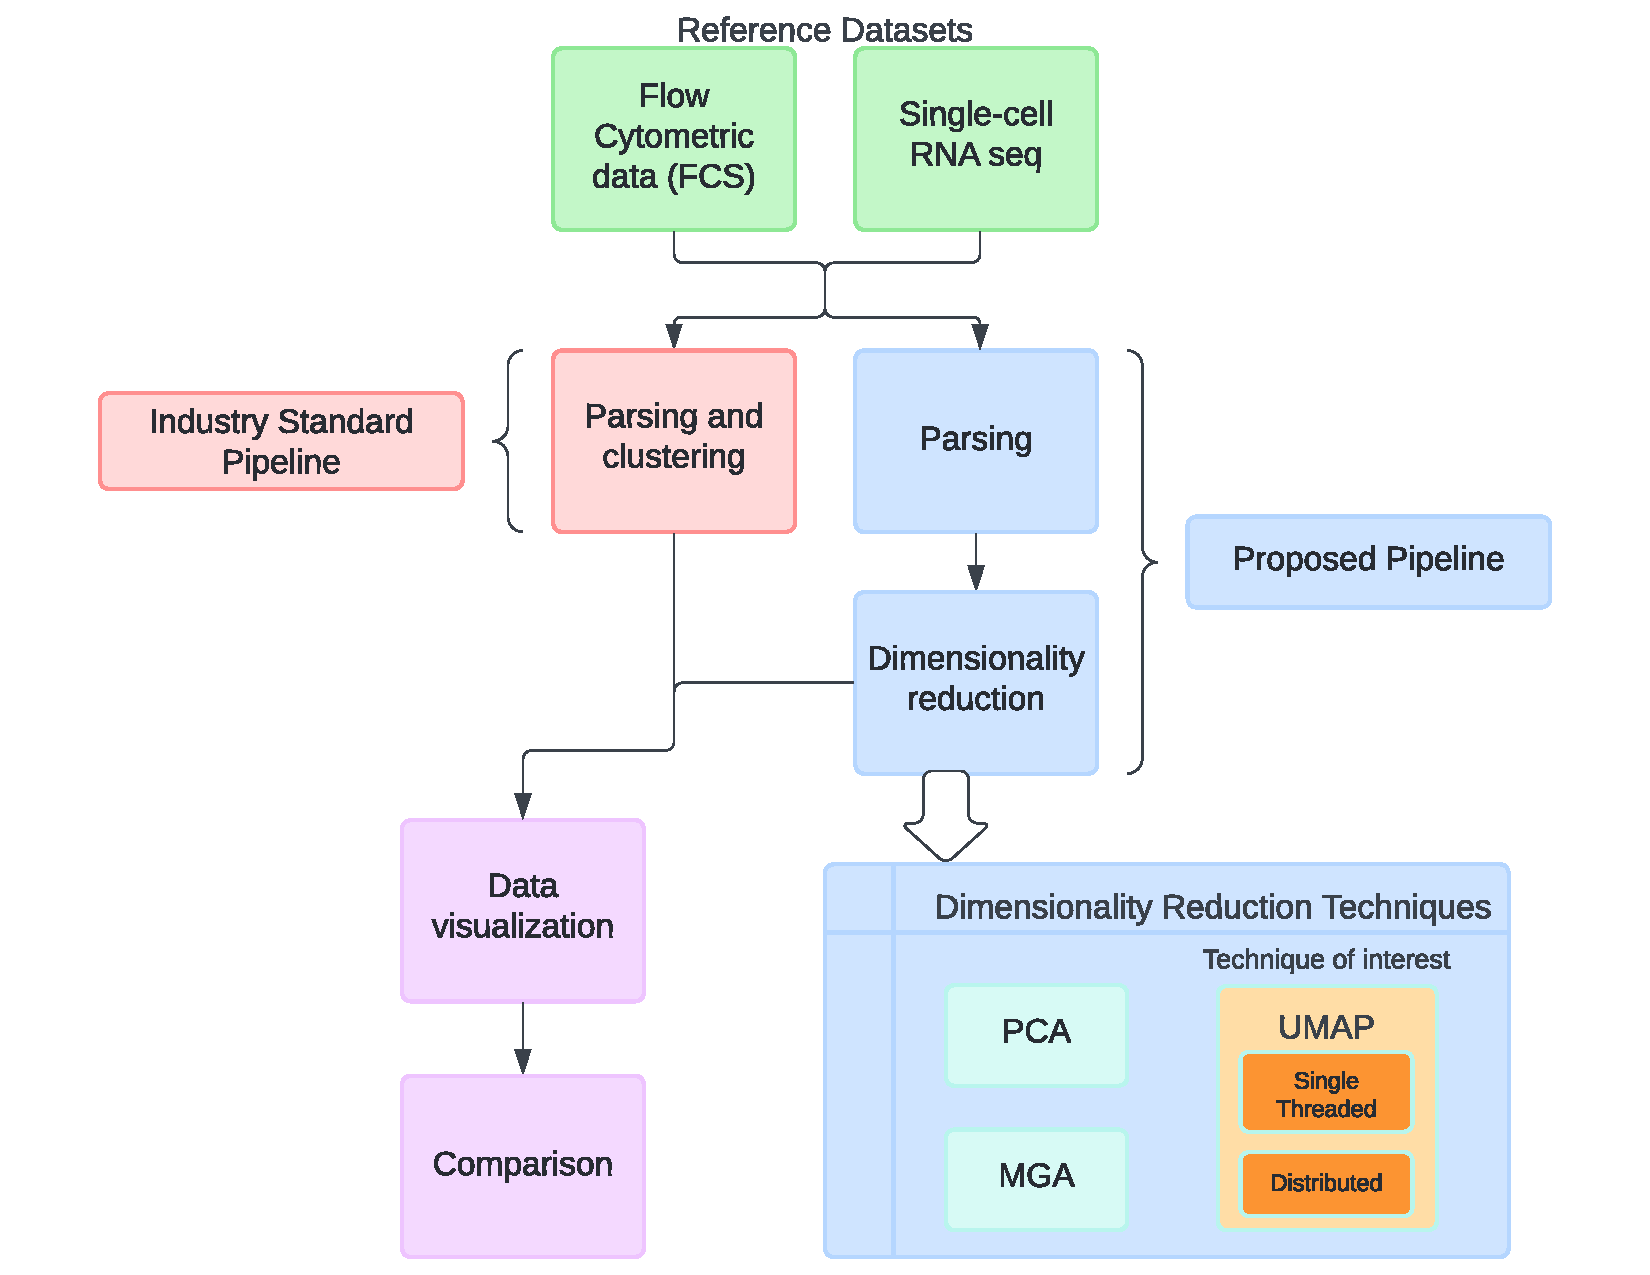
\includegraphics[width=3.4in]{whpc_data_diagram}
    \caption{Data will originate from 3rd-party reference datasets, be analyzed by our pipeline and a reference pipeline, and then our result will be compared against the reference for accuracy.}
    \label{fig:datadiagram}
\end{figure}

% \begin{multicols}{2}

\section{Aims}
\subsection{Implement Strict Data Format}

% Set the big picture central challenge

Poor implimentation of data formats have  % citation needed % demonstration of errors having been introduced

% Discuss methods to demonstrate how the use of strict data formats
% will benefit the field.


Furthermore, it is 

Haskell has repeatedly and reliably been used to unify disperate data formats most notably through the Pandoc system \cite{krijnen2014expand}.

To avoid the possibility of inconsistent data formats, we will write a parser with static type definitions and a strictly defined serialization format. This will feed into a statically typed core framework in Haskell allowing for the guarantees in performance. This framework will make it possible to rely on datatypes thus preventing complex interactions between data sources.

% Standardizing data formats. Different centres generate data in
% different formats, and some analysis tools require data to be in
% particular formats or require different types of data to be linked
% together. Thus, time is wasted reformatting and re-integrating data
% multiple times during a single analysis. For example,
% next-generation sequencing companies do not deliver raw sequencing
% data in a format common to all platforms, as there is no
% industry-wide standard beyond simple text files that include the
% nucleotide sequence and the corresponding quality values. As a
% result, carrying out sequence analyses across different platforms
% requires tools to be adapted to specific platforms.

% It is therefore crucial to develop interoperable sets of analysis
% tools that can be run on different computational platforms depending
% on which is best suited for a given application, and then stitch
% those tools together to form analysis pipelines.

% Modelling the results. A primary goal for biological researchers is
% to integrate diverse, large-scale data sets to construct models that
% can predict complex phenotypes such as disease. As mentioned above,
% constructing predictive models can be computationally
% demanding. Consider, for example, reconstructing Bayesian networks
% using large-scale DNA or RNA variation, DNA–protein binding, protein
% interaction, metabolite and other types of data. As the scales and
% diversity of the data grow, this type of modelling will become
% increasingly important for representing complex systems and
% predicting their behaviour. Computationally, however, the need for
% this type of modelling poses an intense problem that falls into the
% category of NP hard problems9 (Fig. 1). Finding the best Bayesian
% network by searching through all possible networks is a complex
% process; this is true even in cases in which there are only ten
% genes (or nodes), given that there would be in the order of 1018
% possible networks. As the number of nodes increases, the number of
% networks to consider grows superexponentially. The computational
% environments that are required to organize vast amounts of data,
% build complex models from them and then enable others to interpret
% their data in the more informative context of existing models are
% beyond what is available today in the life sciences.

In order to enhance the efficiency and scalability, we will use Haskell's strengths as a functional language that promote parallelism and concurrency. 
It has already been demonstrated that Haskell is an extremely reliable choice for complex systems requiring parallelism. % insert citation regarding facebook's graph search
Popular packages have been developed, which we will be able to leverage. % which popular packages are good candidates? 
Because code in Haskell prevents mutability, while also providing enhanced correctness guarantees to instill confidence in analysis outcomes. By bridging this gap in the analytical toolkit available to researchers, we can facilitate the exploration of high-dimensional datasets with greater efficiency, reliability, and scalability, potentially leading to advancements in scientific research. 

% This formula is proven to work. 


% `Aim 1: To improve the identification of post-translational
% modifications and amino acid substitutions on proteins by
% combiningtop-down and bottom-up mass spectrometry data, we will
% enhance our PROCLAME software to use a Markov chain Monte Carlo
% algorithm that can incorporate: a) intact-mass mass data from
% top-down analysis, b) peptide data from bottom-up analysis, and c)
% context-sensitive rules that use but are not limited by knowledge of
% where modifications are likely to occur. We will further enhance the
% program’s assessment of modification frequency by ongoing analyses
% of protein databases like UniProt5.' Here, I have underlined the Why
% and boldfaced the How. Again, for a good aim, it must have both.''

Statically-typed parser for ensuring data conformity to standards specifically using scRNAseq datasets and flow cytometric datasets. Optional: parsing raw scRNA reads for quality metrics demonstrating reliable scalability for big data.

The use of static typing is because despite what it says in \cite{Schadt_2010}, cloud computing does not inherently address the issues involved with the failure of consistent data formats, and our integration of testings will allow for the detection of datatype mismatches that can plague pipeline outputs with occult mistakes if errors in data parsing are not detected. Erroneous statement follows:

\begin{quotation}
  Cloud computing and heterogeneous computational environments are relatively recent inventions that address many of the limitations mentioned above relating to data transfer, access control, data management, standardization of data formats and advanced model building
\end{quotation}

Two different data types is prompted by the \cite{Schadt_2010} article:

\begin{quotation}
A number of challenges are posed by large-scale data analysis, including data transfer (bringing the data and computational resources together), controlling access to the data, managing the data, standardizing data formats and integrating data of multiple different types to accurately model biological systems.  
\end{quotation}

2. Haskell-implemented dimensionality reduction demonstrated to work on sample data

\begin{quote}
Knowing the parallelization of the analysis algorithms enables a more efficient solution to a computational problem by distributing tasks over many computer processors. The types of parallelism can be classified into two broad categories: loosely coupled (or coarse-grained) parallelism and tightly coupled (or fine-grained) parallelism, each benefiting from different types of computational platforms, depending on the problem of interest.  
\end{quote}

3. Demonstrated ability for Haskell dimensionality reduction tool to handle big data at the level of greater than one terabyte

``Biological research is becoming ever more information-driven, with individual laboratories now capable of generating terabyte scales of data in days. Super-computing resources will be increasingly needed to get the most from the big data sets that researchers generate or analyse.''

4. Parallel Processing

5. Show that our work improves on the state of the art by producing output that has enhanced parallel processing, better error handling, and greater reliability while agreeing with the results of our reference standard \cite{vieth2019systematic}.


1. lit review
2. parsing phase
3. single-threading phase
4. parallelism phase
5. final testing phase

\section{Timeline}
% \begin{multicols}{2}
\begin{enumerate}
    \item Planning Phase (August 2024)
\begin{itemize}
    \item Literature review in UMAP, functional programming in Haskell, and existing frameworks for high dimensional data analysis.
    \item Outline the specific requirements and objectives of the proposed framework.
    \item Conceptualize design architecture and data structures for the UMAP framework in Haskell.
\end{itemize}
\item Implementation Phase (September-October 2024)
\begin{itemize}
    \item Code the core functionalities of the UMAP algorithm in Haskell (single-threaded version).
    \item Develop initial methods to verify the correctness and functionality of implemented components.
\end{itemize}
\item Implementation Phase 2 (November--December 2025)
\begin{itemize}
    \item Continue development of code to create a distributed UMAP version.
    \item Explore parallel processing techniques and libraries in Haskell for potential integration into the framework.
\end{itemize}
\item Optimization Phase (December--February 2025)
\begin{itemize}
    \item Optimize for efficiency and standardize data types based on application.
    \item Conduct performance testing on sample data to assess speed and resource utilization (compare to industry standard).
\end{itemize}
\item Finalization Phase (February–-March 2025)
\begin{itemize}
    \item Polishing API.
    \item Final testing, identify and resolve bugs.
    \item Prepare research paper for the project.
\end{itemize}
\end{enumerate}
% \end{multicols}
\subsection{Resources}
% Should probably include a justification. E.g, we need to demonstrate % parallelism in our program such that it distributes across threads, CPUs, and GPUs. Therefore, we need at least 2 GPUs. We might get bonus points for being familiar with the HiPerGator architecture for planning our performance requirements.
% Justify storage requirements: what dataset do we want to be looking at?

To evaluate the performance of our code we will be using single cell RNA seq and flow cytometric data in order to demonstrate that our framework can work on a variety of data types. 

% \begin{multicols}{2}
\subsubsection{Dataflow diagram}

\begin{enumerate}
\item Data sources (scRNAseq, flow data)
\item Stages of processing (our pipeline)
\item Stages of processing (reference standard)
\item Reconciliation (comparing ours to reference)
\item Downstream applications (generic block)
\end{enumerate}

\subsubsection{Requirements}

\begin{itemize}
    \item CPUs: 8
    \item GPUs: 2
    \item Storage: 2 terabytes
\end{itemize}
% \end{multicols}
\printbibliography
\end{document}
